\documentclass{article}
\usepackage[utf8]{inputenc}

\title{Exam 2 Written}
\author{Benny Chen}
\date{\today}

\usepackage{color}
\usepackage{amsthm}
\usepackage{amssymb} 
\usepackage{amsmath}
\usepackage{listings}
\usepackage{xcolor}
\usepackage{listings}
\usepackage{graphicx}
\usepackage{enumitem}
\usepackage{pdfpages}
\usepackage[hidelinks]{hyperref}

\definecolor{codegreen}{rgb}{0,0.6,0}
\definecolor{codegray}{rgb}{0.5,0.5,0.5}
\definecolor{codepurple}{rgb}{0.58,0,0.82}
\definecolor{backcolour}{rgb}{0.95,0.95,0.92}

\lstdefinestyle{mystyle}{
    backgroundcolor=\color{backcolour},   
    commentstyle=\color{codegreen},
    keywordstyle=\color{magenta},
    numberstyle=\tiny\color{codegray},
    stringstyle=\color{codepurple},
    basicstyle=\ttfamily\footnotesize,
    breakatwhitespace=false,         
    breaklines=true,                 
    captionpos=b,                    
    keepspaces=true,                 
    numbers=left,                    
    numbersep=5pt,                  
    showspaces=false,                
    showstringspaces=false,
    showtabs=false,                  
    tabsize=2
}

\lstset{style=mystyle}

\begin{document}

\maketitle

\section*{Q1 Support Vector Machine}
Suppose we have a hard-margin SVM trained upon a set of data points. If we add new features to these sample points (while retaining all the original features; say, an original data point [a, b, c] becomes [a, b, c, d, e] where d and e can be any numbers), can the optimal $|| w_{new} ||$ in the altered SVM be greater than the optimal $||w_{old}||$in the original SVM?
\\
Can it be smaller?
\\
Can it be the same?
\\
\textbf{Explain why and most of the points will be for your explanation.}

For a hard-margin SVM, if we add new features to a sample of points, the optimal $||w_{new}||$ can be greater, smaller, and the same as the optimal $||w_{old}||$ in the original SVM. This entierly depends on the new features added. If the new features affect the weight postivley or negativley depends on what the new features and weights are. The new weights can change in either direction or stay the same. The only thing that we would know is that there are more datapoints now and are more complex.



\section*{Q2 Principal Component Analysis}

\begin{center}
    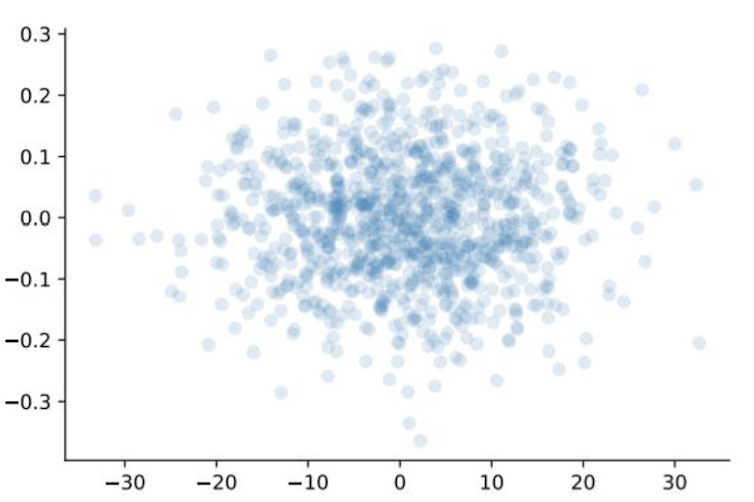
\includegraphics[scale=0.5]{q2.png}
\end{center}

The above are 1,000 sample points drawn from a two-dimensional multivariate normal distribution.
Which of the following matrices could (without extreme improbability) be the covariance matrix of the distribution? Pay attention to the numbers on the axes!

\textbf{Please provide brief explanation regarding your option and why others are not possible.}

\begin{enumerate}[label=(\alph*)]
    \item $ \Sigma =
    \begin{bmatrix}
        100 & 0 \\
        0 & 0.01    
    \end{bmatrix}$
    \item $ \Sigma =
    \begin{bmatrix}
        10 & 0 \\
        0 & 0.1
    \end{bmatrix}$
    \item $ \Sigma =
    \begin{bmatrix}
        1 & 0 \\
        0 & 1
    \end{bmatrix}$
    \item $ \Sigma =
    \begin{bmatrix}
        -10 & 0 \\
        0 & -0.1
    \end{bmatrix}$
    \item None of the above
\end{enumerate}

From the graph we can see that the data is oreinted around the center of the origin and the datapoints are flat and spread out. This shows that there is zero or negligible covariance. This makes our covariance matrix 
\begin{equation}
    \Sigma =
    \begin{bmatrix}
        v_x & 0 \\
        0 & v_y
    \end{bmatrix}
\end{equation}
We can now find the variance of the x and y axis to complete the matrix. The variance is the spread of the datapoints. From the spread we can see that it's flat shaped making the variance of the x axis greater than the y axis. This makes c and d not possible. We can also see that it can't be a because the variance is out the range of the data. This leaves us with b which we can conclude as the answer due to it being in the range of the data and the variance of the x axis being greater than the y axis.

\section*{Q3 Page Rank}
\begin{center}
    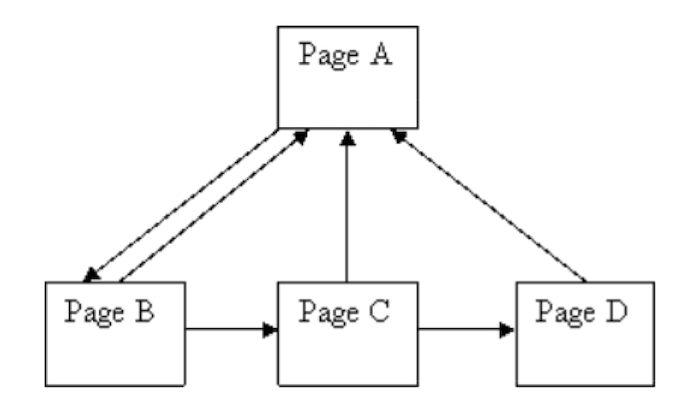
\includegraphics[scale=0.5]{q3.png}
\end{center}

Regarding the above webpages and their mutual connections, please derive the page ranks (assuming all ranks are 1 initially) after the convergence is observed.

\textbf{Warnings: be extremely careful if you have the stochastic weights which do not sum up to exact 1 per webpage. Please make sure the input has the weights per web page that sum up to exact 1! (You will know what I am talking about if you really code above).}
\\
First we make a Stochastic Matrix for the graph which we get:
\begin{table}[h]
    \begin{tabular}{lllll}
        & A & B   & C   & D \\
    A & 0 & 0.5 & 0.5 & 1 \\
    B & 1 & 0   & 0   & 0 \\
    C & 0 & 0.5 & 0   & 0 \\
    D & 0 & 0   & 0.5 & 0
    \end{tabular}
    \centering
\end{table}
\\
With all columns summing up to 1. We then plug this into the PageRank formula: 
\begin{equation}
    r = M*r
\end{equation}
\\
Where $r$ is the sum of the columns of the matrix and $M$ is the Stochastic Matrix. We then solve for $r$:
\begin{equation}
    r = 
    \begin{bmatrix}
        0 & 0.5 & 0.5 & 1 \\
        1 & 0 & 0 & 0 \\
        0 & 0.5 & 0 & 0 \\
        0 & 0 & 0.5 & 0
    \end{bmatrix}
    * 
    \begin{bmatrix}
        1 \\
        1 \\
        1 \\
        1
    \end{bmatrix}
\end{equation}
This gives us the following:
\begin{equation}
    r = 
    \begin{bmatrix}
        2 \\
        1 \\
        0.5 \\
        0.5
    \end{bmatrix}
\end{equation}
Which we then keep plugging into the formula until we see a convergence. We then get the following:
\begin{equation}
    \begin{bmatrix}
        1.45460486 \\
        1.45.446849 \\
        0.72732258 \\
        0.36360407
    \end{bmatrix}
\end{equation}

\end{document}